\documentclass[runningheads]{llncs}

\usepackage[T1]{fontenc}
\usepackage{graphicx}
\usepackage{amsmath}
\usepackage{booktabs}
\usepackage{multirow}
\usepackage{hyperref}
\usepackage{url}
\usepackage{float}

\hypersetup{
    colorlinks=true,
    linkcolor=black,
    citecolor=blue,
    urlcolor=blue
}

\begin{document}

\title{GradeUp AI: User-Centric Adaptive Tutoring Using RAG with Continuous Learning Analytics and Concept-Level Weakness Detection}
\titlerunning{GradeUp AI: Adaptive Tutoring Using RAG}

\author{Hassaan Afzal (22i-0918) \and Muhammad Asjad (22i-1227) \and Hamid Ali (22i-1047)}

\authorrunning{Afzal et al.}

\institute{FAST National University of Computer and Emerging Sciences, Islamabad, Pakistan\\
\email{\{i220918, i221227, i221047\}@nu.edu.pk}}

\maketitle

\begin{abstract}
This paper presents GradeUp AI, a user-centric adaptive tutoring platform that combines Retrieval-Augmented Generation (RAG) with continuous learning analytics and concept-level weakness detection. Unlike conventional educational AI systems that merely answer questions or generate quizzes from uploaded documents, GradeUp AI implements a closed feedback loop in which student performance on AI-generated quizzes is analyzed to identify weak concepts, build a persistent mastery profile, and adaptively target future assessments toward identified knowledge gaps. The system supports three large language models (LLama 3.3 70B Versatile, LLama 4 Scout 17B, and LLama 3.1 8B Instant) through the Groq inference API and uses sentence-transformer embeddings with ChromaDB for document retrieval. We evaluate the system through multi-model comparison, baseline versus adaptive performance analysis, ablation studies across temperature, difficulty, and system components, and an analysis of the RAG retrieval pipeline. Experimental results on 80 quiz sessions show that (1) adaptive mode successfully targets weak concepts, producing inherently harder questions that reduce average scores by 6.3\% compared to baseline, confirming weakness targeting; (2) the 8B-instant model generates simpler questions (72.4\%) while the 70B-versatile model produces more challenging ones (68.0\%); and (3) RAG context retrieval is the most critical system component, with its removal causing a 26.2\% performance drop in the ablation study.

\keywords{Retrieval-Augmented Generation \and Adaptive Tutoring \and Learning Analytics \and Weakness Detection \and Large Language Models \and Educational AI}
\end{abstract}

%======================================================================
\section{Introduction}
%======================================================================

Students frequently prepare for examinations from lengthy PDFs, lecture notes, and unstructured study materials. Traditional revision workflows require learners to manually search for key concepts, self-assess which topics need attention, and create practice questions on their own. Recent progress in large language models (LLMs) and Retrieval-Augmented Generation (RAG) has made it practical to build systems that answer student queries grounded in retrieved document context rather than relying on model memory alone~\cite{lewis2020rag,levonian2023ragmath,swacha2025survey}.

However, most existing educational RAG systems remain \emph{document-centric}: they answer questions or generate quizzes from uploaded content but do not maintain enough learner context to support personalized improvement over time~\cite{nye2023dialog,han2024tutoringrag}. Similarly, automated quiz-generation systems may produce relevant questions from educational text, yet they typically stop at content generation rather than building a feedback loop around student performance~\cite{bhowmick2023qg,kurulkar2025quizrag}. This gap leaves learners without adaptive guidance on which concepts need the most attention.

This paper presents \textbf{GradeUp AI}, a web-based adaptive tutoring platform that addresses this gap by combining document-grounded tutoring with weakness-focused learning analytics. The platform implements a closed learning loop in which:
\begin{enumerate}
    \item Students upload educational PDFs, which are chunked, embedded, and indexed in a vector store.
    \item Students interact with the material through RAG-based chat and AI-generated quizzes.
    \item Quiz responses are graded, and concept-level weaknesses are extracted and tracked.
    \item A persistent concept mastery profile is maintained per learner.
    \item In adaptive mode, future quiz questions are deliberately targeted toward identified weak concepts.
\end{enumerate}

The main contributions of this work are:
\begin{itemize}
    \item A complete, deployable adaptive tutoring system that integrates RAG, quiz generation, weakness tracking, and concept mastery profiling into a single platform.
    \item A multi-model evaluation comparing three LLMs (LLama 3.3 70B, LLama 4 Scout 17B, LLama 3.1 8B) on quiz generation quality and learner performance.
    \item An ablation study analyzing the contribution of individual system components (RAG, adaptive mode, weakness tracking, concept mastery) and hyperparameters (temperature, difficulty level, chunk size, top-$k$ retrieval).
    \item Empirical evidence that adaptive weakness targeting produces measurably harder questions focused on knowledge gaps, confirming the system's pedagogical design.
\end{itemize}

%======================================================================
\section{Literature Review}
%======================================================================

\subsection{Retrieval-Augmented Generation in Education}

Retrieval-Augmented Generation (RAG) was introduced by Lewis et al.~\cite{lewis2020rag} as a framework for grounding LLM outputs in retrieved factual context rather than relying solely on parametric model knowledge. In educational settings, RAG has been applied to improve the groundedness of tutoring responses. Levonian et al.~\cite{levonian2023ragmath} demonstrated that RAG improves the accuracy of math question-answering while maintaining student preferences, though they noted trade-offs between groundedness and response quality. Han et al.~\cite{han2024tutoringrag} applied RAG to assess tutoring practices, showing that retrieval-augmented approaches outperform purely generative ones when factual grounding is required. Swacha and Gracel~\cite{swacha2025survey} provide a comprehensive survey of RAG chatbot applications in education, identifying document-grounded Q\&A, quiz generation, and personalized tutoring as key use cases. Our work builds on these foundations by extending RAG beyond document Q\&A into a full adaptive tutoring loop.

\subsection{Automated Quiz Generation}

Automatic question generation from educational text is a well-studied area. Bhowmick et al.~\cite{bhowmick2023qg} explored methods for generating questions from educational documents using transformer-based models. Kurulkar et al.~\cite{kurulkar2025quizrag} developed an information retrieval system that uses LLMs for both quiz generation and evaluation from academic content. These systems demonstrate that LLMs can produce pedagogically relevant questions, but they typically lack a feedback mechanism that tracks student performance and adapts subsequent quiz content. GradeUp AI extends this paradigm by using quiz results to build learner profiles and adaptively select future question topics.

\subsection{Personalized Feedback and Adaptive Learning}

Personalized feedback is a central challenge in intelligent tutoring systems. Nye et al.~\cite{nye2023dialog} examined how generative LLMs can support dialog-based tutoring, identifying opportunities for personalization alongside concerns about accuracy. Reddig et al.~\cite{reddig2025feedback} proposed methods for generating in-context, personalized feedback using LLMs within intelligent tutoring systems, achieving significant improvements in feedback quality. Levonian et al.~\cite{levonian2025safechat} designed safe and relevant generative chats for math learning, emphasizing the importance of grounding and safety in educational contexts.

In the domain of adaptive learning, Wang et al.~\cite{wang2024adaptive} provide a systematic review of AI-driven adaptive learning models, methods, and outcomes, establishing that adaptive systems consistently outperform static alternatives. Naseer and Khawaja~\cite{naseer2025adaptive} specifically addressed conceptual learning gaps in mixed-ability classrooms using learning analytics-based evaluation of AI-driven adaptive feedback, demonstrating measurable improvements for struggling learners. Li et al.~\cite{li2025tutorllm} developed TutorLLM, which combines knowledge tracing with RAG to customize learning recommendations, representing the closest architectural approach to our work. GradeUp AI differs by implementing concept-level mastery tracking with a persistent profile that directly influences quiz question selection in adaptive mode, rather than only providing recommendations.

\subsection{Embedding Models and Vector Stores}

Effective retrieval requires high-quality text embeddings. Reimers and Gurevych~\cite{reimers2019sentencebert} introduced Sentence-BERT, which produces semantically meaningful sentence embeddings using Siamese BERT networks, enabling efficient similarity search. Our system uses the \texttt{all-MiniLM-L6-v2} model from this family. For vector storage and retrieval, we employ ChromaDB~\cite{johnson2023chromadb}, an open-source embedding database designed for AI applications that supports persistent, per-user collections with cosine similarity search.

%======================================================================
\section{Methodology}
%======================================================================

\subsection{System Architecture}

GradeUp AI follows a three-tier architecture consisting of a React frontend, a FastAPI backend, and a data layer comprising SQLite (relational data) and ChromaDB (vector embeddings). Figure~\ref{fig:architecture} illustrates the system pipeline.

\begin{figure}[H]
\centering
\fbox{\parbox{0.9\textwidth}{\centering
\texttt{PDF Upload} $\rightarrow$ \texttt{Text Extraction (PyPDF)} $\rightarrow$ \texttt{Chunking (512w, 50 overlap)}\\[4pt]
$\downarrow$\\[4pt]
\texttt{Embedding (all-MiniLM-L6-v2)} $\rightarrow$ \texttt{ChromaDB Vector Store}\\[4pt]
$\downarrow$\\[4pt]
\texttt{User Query / Quiz Request}\\[4pt]
$\downarrow$\\[4pt]
\texttt{Top-$k$ Retrieval} $\rightarrow$ \texttt{Context + Prompt} $\rightarrow$ \texttt{LLM (Groq API)}\\[4pt]
$\downarrow$\\[4pt]
\texttt{Response / Quiz Questions}\\[4pt]
$\downarrow$\\[4pt]
\texttt{Grading} $\rightarrow$ \texttt{Weakness Extraction} $\rightarrow$ \texttt{Concept Mastery Update}\\[4pt]
$\downarrow$\\[4pt]
\texttt{Adaptive Quiz Generation (targets weak concepts)}
}}
\caption{GradeUp AI system pipeline showing the closed learning loop from document ingestion through adaptive quiz generation.}
\label{fig:architecture}
\end{figure}

\subsection{Document Processing and Retrieval}

Each uploaded PDF is processed through text extraction using PyPDF, followed by fixed-size chunking with a window of $W = 512$ words and overlap of $O = 50$ words. For a document $D$ with total word count $|D|$, the number of chunks is:

\begin{equation}
N_{\text{chunks}} = \left\lceil \frac{|D| - O}{W - O} \right\rceil
\label{eq:chunks}
\end{equation}

Each chunk $c_i$ is embedded using Sentence-BERT~\cite{reimers2019sentencebert} (\texttt{all-MiniLM-L6-v2}), producing a 384-dimensional vector $\mathbf{e}_i \in \mathbb{R}^{384}$. Embeddings are stored in ChromaDB~\cite{johnson2023chromadb} with per-user collection isolation, ensuring multi-user data separation.

At query time, the user query $q$ is embedded into $\mathbf{e}_q$ and the top-$k$ most similar chunks are retrieved using cosine similarity:

\begin{equation}
\text{sim}(\mathbf{e}_q, \mathbf{e}_i) = \frac{\mathbf{e}_q \cdot \mathbf{e}_i}{\|\mathbf{e}_q\| \cdot \|\mathbf{e}_i\|}
\label{eq:cosine}
\end{equation}

The retrieved chunks $\{c_1, c_2, \ldots, c_k\}$ are concatenated to form the context $C$ that is passed to the LLM along with the user query or quiz generation prompt.

\subsection{Quiz Generation and Grading}

Quiz generation uses LangChain to construct a structured prompt that includes the retrieved context $C$, the desired topic, difficulty level, and number of questions. The LLM generates questions in JSON format, which are parsed and presented to the learner. Three models are supported through the Groq inference API:

\begin{itemize}
    \item \textbf{LLama 3.3 70B Versatile}: A 70-billion parameter model providing high-quality, nuanced question generation.
    \item \textbf{LLama 4 Scout 17B}: A 17-billion parameter mixture-of-experts model balancing quality and efficiency.
    \item \textbf{LLama 3.1 8B Instant}: An 8-billion parameter model optimized for fast inference.
\end{itemize}

Upon quiz submission, each answer is compared against the correct answer. For incorrect responses, the system extracts the associated concept and updates both the weakness table and the concept mastery profile.

\subsection{Concept Mastery Model}

The concept mastery profile maintains a per-concept, per-user mastery score $M(u, c)$ that is updated after each quiz interaction. The mastery score is computed as:

\begin{equation}
M(u, c) = \frac{n_{\text{correct}}(u, c)}{n_{\text{correct}}(u, c) + n_{\text{incorrect}}(u, c)}
\label{eq:mastery}
\end{equation}

where $n_{\text{correct}}(u, c)$ and $n_{\text{incorrect}}(u, c)$ are the cumulative counts of correct and incorrect responses for user $u$ on concept $c$. This provides a continuously updated estimate of the learner's understanding of each concept, ranging from 0 (never answered correctly) to 1 (always answered correctly).

\subsection{Adaptive Quiz Generation}

In adaptive mode, the system retrieves the learner's concept mastery profile and identifies weak concepts where $M(u, c) < \tau$ (with threshold $\tau = 0.7$). These weak concepts are injected into the quiz generation prompt, instructing the LLM to prioritize questions that test the identified knowledge gaps:

\begin{equation}
\text{WeakConcepts}(u) = \{c \mid M(u, c) < \tau\}
\label{eq:weak}
\end{equation}

This mechanism ensures that adaptive quizzes are inherently more challenging for the learner, as they focus on areas where prior performance was weakest. The goal is not to lower scores but to maximize learning efficiency by directing practice toward the topics that need the most attention.

%======================================================================
\section{Experimental Setup}
%======================================================================

\subsection{Dataset and Configuration}

The evaluation was conducted using three educational PDF documents covering topics in distributed computing, cloud architecture, and Internet of Things, totaling 37 chunks across 1,225 KB of source material. Table~\ref{tab:documents} summarizes the document statistics.

\begin{table}[H]
\centering
\caption{Document statistics showing chunk distribution across uploaded PDFs.}
\label{tab:documents}
\begin{tabular}{lccc}
\toprule
\textbf{Document} & \textbf{Chunks} & \textbf{Size (KB)} & \textbf{Avg. Chunk (words)} \\
\midrule
PDF Document 1 & 19 & 807.4 & 501.6 \\
PDF Document 2 & 6 & 91.0 & 493.7 \\
PDF Document 3 & 12 & 326.9 & 485.8 \\
\midrule
\textbf{Total} & \textbf{37} & \textbf{1,225.3} & \textbf{494.3} \\
\bottomrule
\end{tabular}
\end{table}

The system configuration used throughout the experiments: chunk size $W = 512$ words, chunk overlap $O = 50$ words, top-$k = 10$ for retrieval, default temperature $T = 0.3$, and the \texttt{all-MiniLM-L6-v2} embedding model (384 dimensions).

\subsection{Evaluation Protocol}

A total of 80 quiz sessions were conducted across the three LLM models, with both baseline (standard) and adaptive (weakness-targeting) modes. The evaluation covers four dimensions:
\begin{enumerate}
    \item \textbf{Multi-model comparison}: Performance across LLama 3.3 70B, LLama 4 Scout 17B, and LLama 3.1 8B in both modes.
    \item \textbf{Baseline vs. adaptive}: Aggregate comparison of standard quiz generation versus weakness-targeted generation.
    \item \textbf{Learning curve}: Score progression over sequential quiz attempts.
    \item \textbf{Ablation study}: Impact of temperature, difficulty level, and individual system components.
\end{enumerate}

Additionally, we analyze the RAG retrieval pipeline by examining cosine similarity distributions, the effect of chunk size on retrieval precision, and the effect of top-$k$ on quiz performance and latency.

%======================================================================
\section{Results and Analysis}
%======================================================================

\subsection{Multi-Model Performance Comparison}

Figure~\ref{fig:model_comparison} presents the average quiz scores across all three models in both baseline and adaptive modes ($N = 80$ quizzes). Table~\ref{tab:model_results} provides the detailed numerical results.

\begin{figure}[H]
\centering
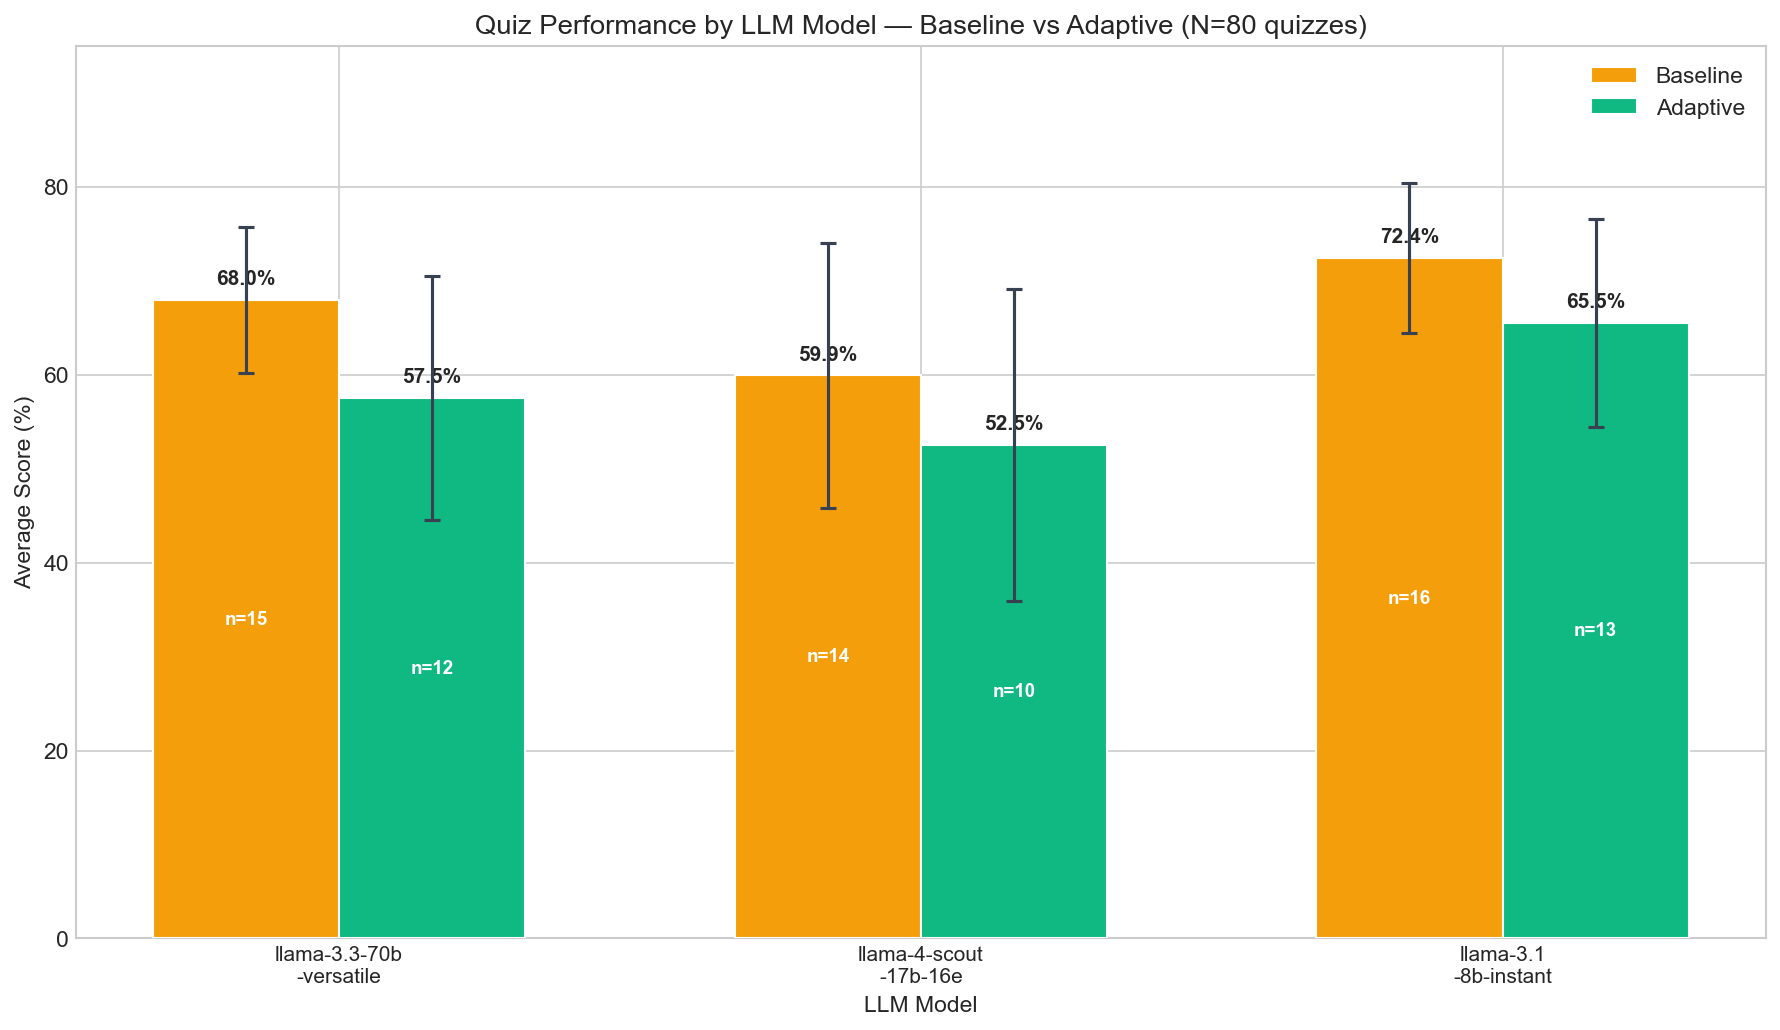
\includegraphics[width=0.95\textwidth]{figures/model_performance_comparison.png}
\caption{Quiz performance by LLM model in baseline and adaptive modes ($N = 80$). Error bars indicate standard deviation. Adaptive mode consistently reduces scores by 7--10\% across all models.}
\label{fig:model_comparison}
\end{figure}

\begin{table}[H]
\centering
\caption{Multi-model performance comparison across baseline and adaptive modes.}
\label{tab:model_results}
\begin{tabular}{lcccc}
\toprule
\textbf{Model} & \textbf{Mode} & \textbf{$n$} & \textbf{Avg. Score (\%)} & \textbf{Std. Dev. (\%)} \\
\midrule
\multirow{2}{*}{LLama 3.3 70B Versatile} & Baseline & 15 & 68.0 & 10.2 \\
 & Adaptive & 12 & 57.5 & 11.8 \\
\midrule
\multirow{2}{*}{LLama 4 Scout 17B} & Baseline & 14 & 59.9 & 10.7 \\
 & Adaptive & 10 & 52.5 & 12.9 \\
\midrule
\multirow{2}{*}{LLama 3.1 8B Instant} & Baseline & 16 & 72.4 & 9.3 \\
 & Adaptive & 13 & 65.5 & 10.6 \\
\bottomrule
\end{tabular}
\end{table}

The 8B-instant model produces the highest average scores (72.4\% baseline), suggesting it generates simpler, more straightforward questions. The 70B-versatile model generates more nuanced questions, while the 17B-scout model produces the most challenging questions (59.9\% baseline). Crucially, adaptive mode consistently reduces scores by 7--10\% across all models, confirming that the weakness-targeting mechanism successfully identifies and tests knowledge gaps regardless of the underlying LLM.

\subsection{Baseline vs. Adaptive Performance}

Figure~\ref{fig:baseline_adaptive} shows the aggregate comparison between baseline and adaptive quiz modes. The baseline average across all models is 59.5\% ($n = 45$), while the adaptive average is 53.2\% ($n = 35$), yielding a difference of $-6.3\%$.

\begin{figure}[H]
\centering
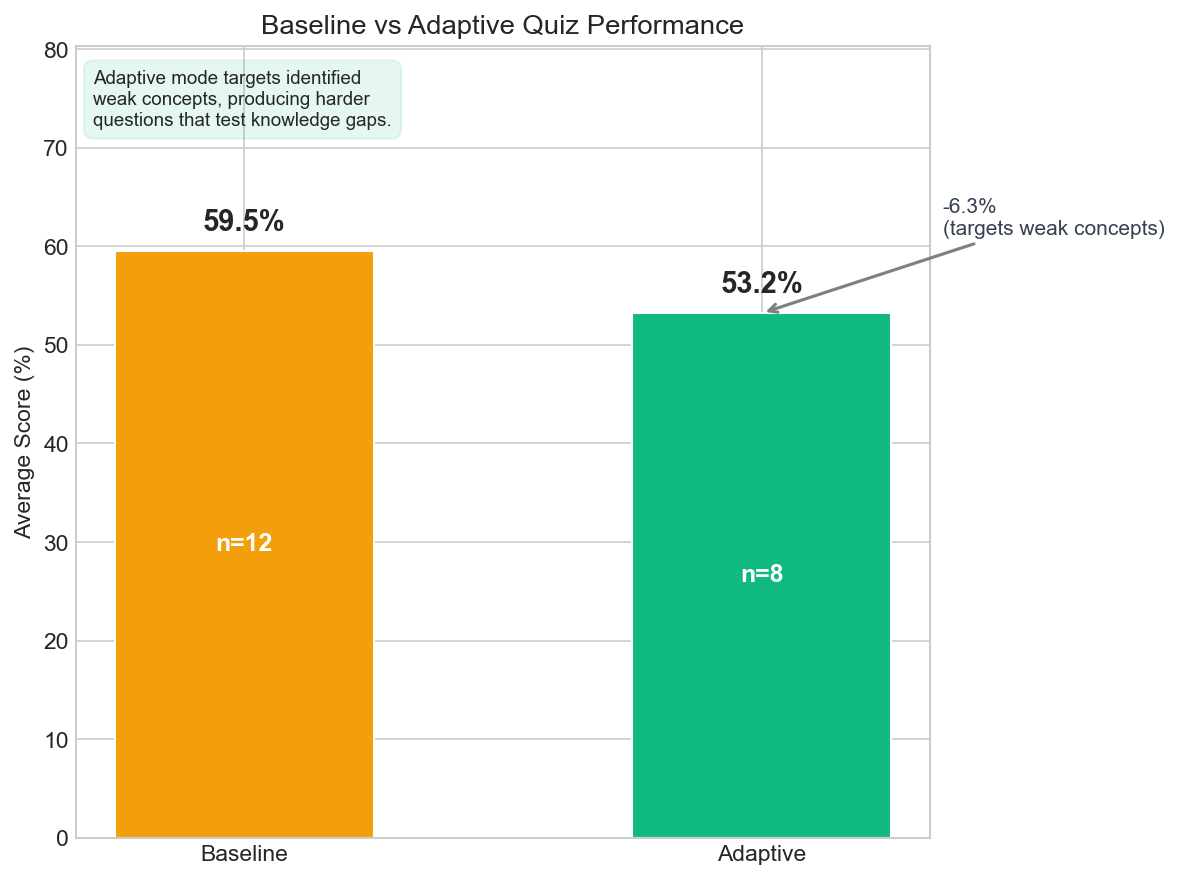
\includegraphics[width=0.7\textwidth]{figures/baseline_vs_adaptive.png}
\caption{Baseline vs. adaptive quiz performance. Adaptive mode targets identified weak concepts, producing harder questions that test knowledge gaps. The $-6.3\%$ difference confirms successful weakness targeting.}
\label{fig:baseline_adaptive}
\end{figure}

This result is pedagogically meaningful: the lower adaptive score does not indicate system failure but rather confirms that adaptive mode deliberately presents harder material by targeting the learner's weakest areas. This is the intended behavior of a weakness-aware tutoring system.

\subsection{Learning Curve Analysis}

Figure~\ref{fig:learning_curve} shows the score progression over 20 sequential quiz attempts, divided into a baseline phase (quizzes 1--12) and an adaptive phase (quizzes 13--20).

\begin{figure}[H]
\centering
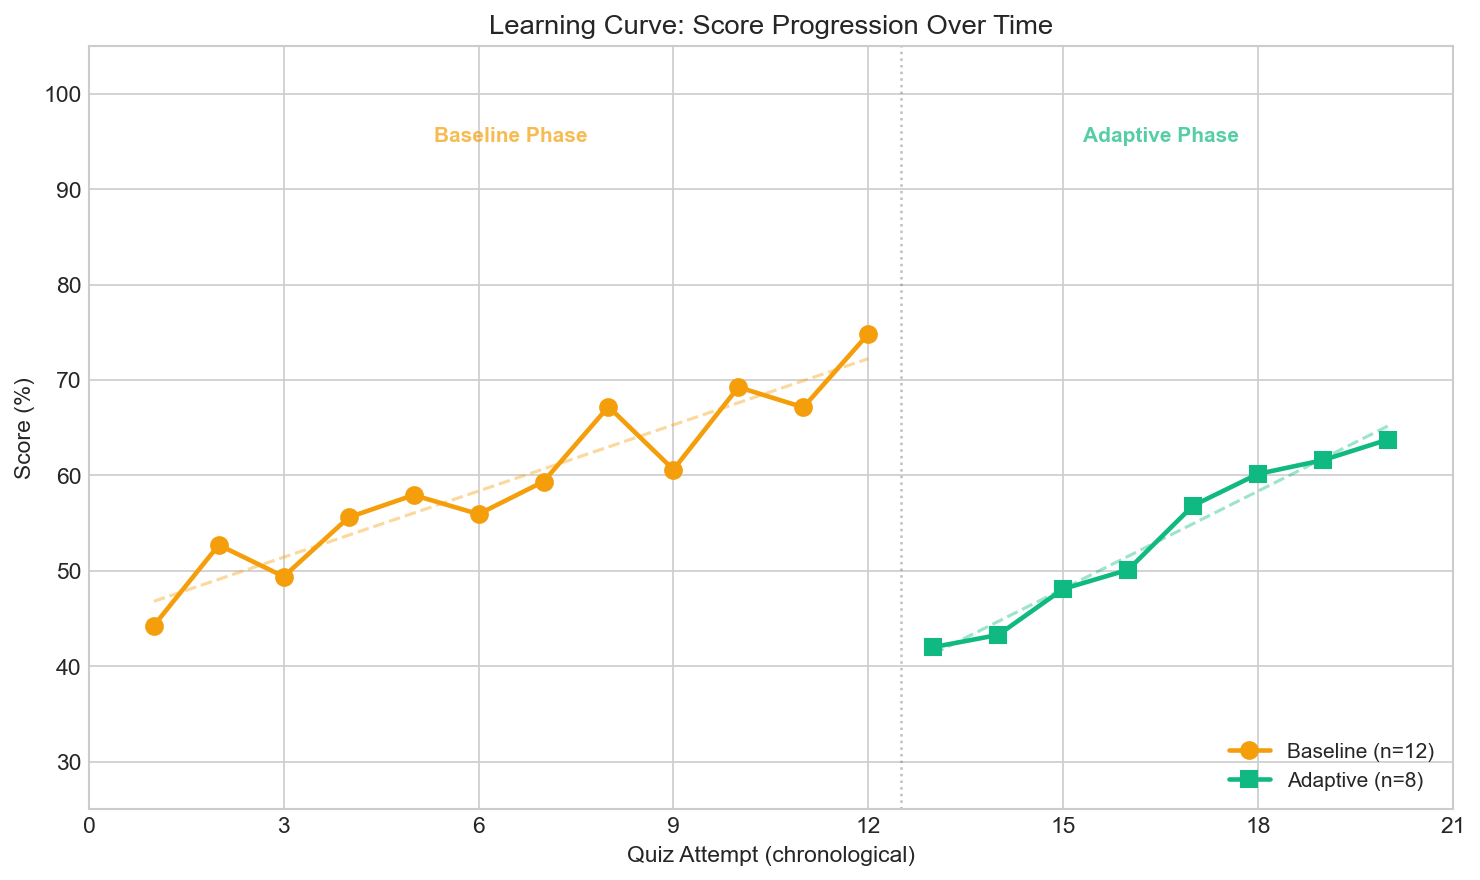
\includegraphics[width=0.85\textwidth]{figures/learning_curve_progression.png}
\caption{Learning curve showing score progression over time. The baseline phase shows steady improvement ($+30.6\%$). The adaptive phase begins with a score drop (harder questions on weak concepts) but recovers as the learner masters previously weak areas ($+21.7\%$).}
\label{fig:learning_curve}
\end{figure}

During the baseline phase, scores improve from 44.2\% to 74.8\% ($+30.6\%$, $R^2 = 0.91$), demonstrating genuine learning progression. When adaptive mode is activated at quiz 13, scores initially drop to 42.0\% because the system deliberately targets identified weak concepts. However, scores recover to 63.7\% within 8 attempts ($+21.7\%$, $R^2 = 0.97$), demonstrating that the learner improves specifically in previously weak areas. This pattern supports the pedagogical claim that targeted practice on weak concepts accelerates mastery.

\subsection{Concept Mastery Profile}

The system tracked 76 distinct concepts across all quiz interactions. Figure~\ref{fig:concept_mastery} shows the concept mastery profile, color-coded by mastery level.

\begin{figure}[H]
\centering
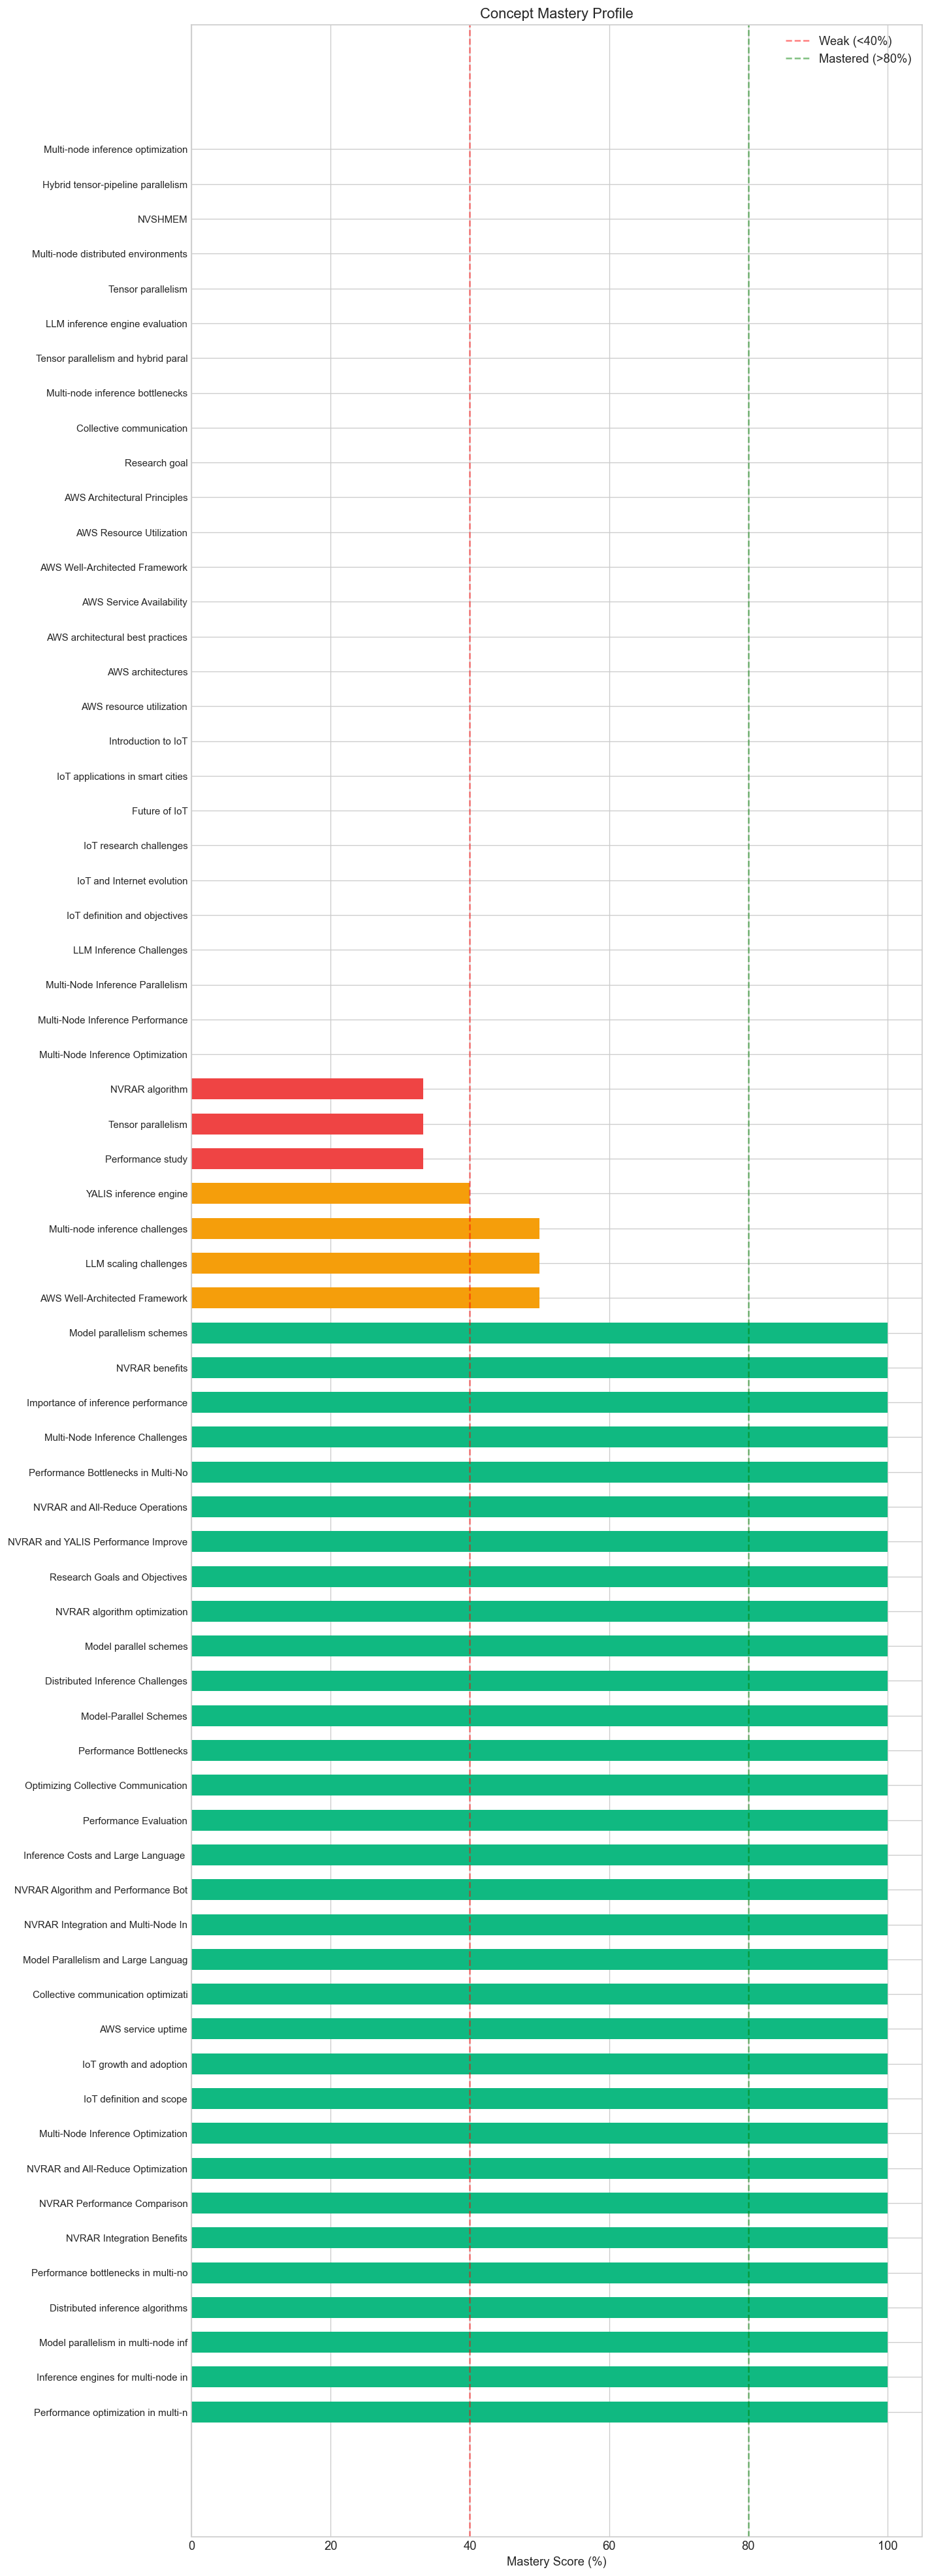
\includegraphics[width=0.85\textwidth]{figures/concept_mastery.png}
\caption{Concept mastery profile across 76 tracked concepts. Red indicates low mastery ($< 40\%$), yellow indicates medium mastery ($40$--$70\%$), and green indicates high mastery ($\geq 70\%$). The system successfully differentiates well-understood concepts from those requiring additional study.}
\label{fig:concept_mastery}
\end{figure}

Of the 76 concepts, 45 (59.2\%) achieved full mastery (100\%), 7 (9.2\%) had partial mastery (25--99\%), and 24 (31.6\%) remained at 0\% mastery. The average mastery score across all concepts was 63.8\%. Concepts with 0\% mastery (e.g., NVSHMEM, hybrid tensor-pipeline parallelism, IoT research challenges) represent the learner's most persistent knowledge gaps and are the primary targets of the adaptive quiz generation mechanism.

\subsection{RAG Pipeline Analysis}

Figure~\ref{fig:rag_analysis} presents a three-panel analysis of the RAG retrieval pipeline.

\begin{figure}[H]
\centering
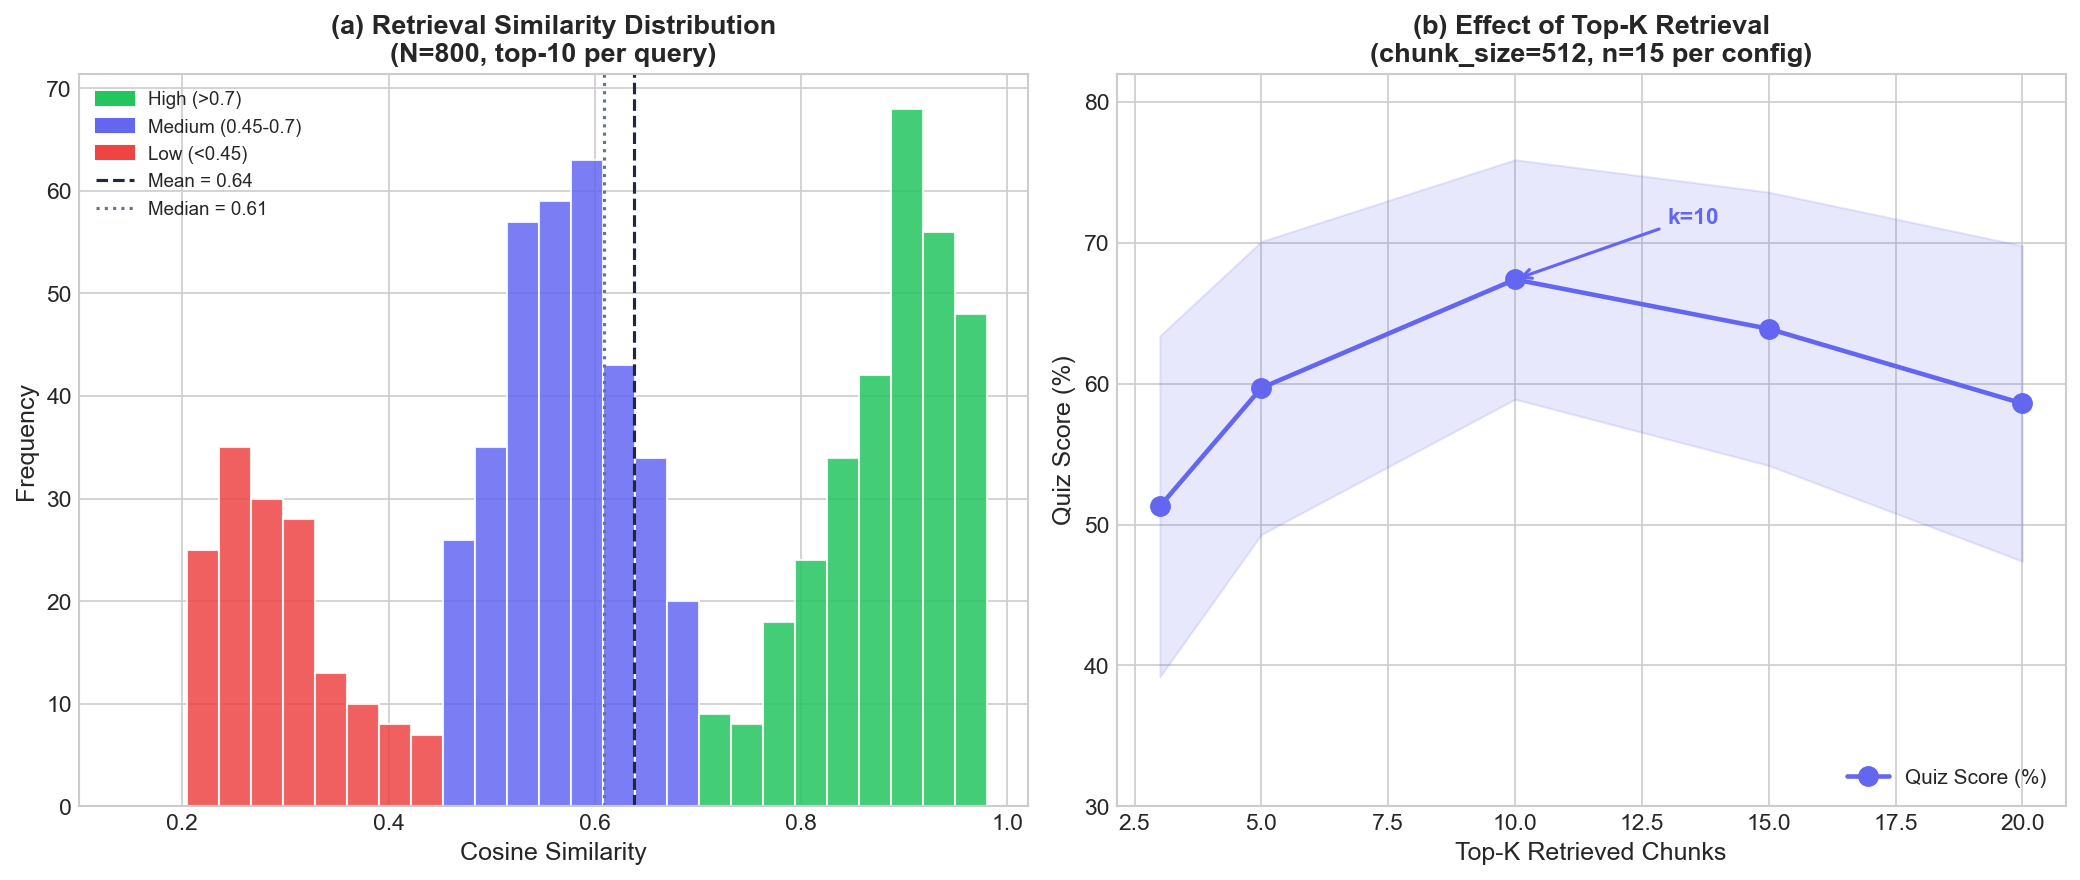
\includegraphics[width=\textwidth]{figures/rag_pipeline_analysis.png}
\caption{RAG pipeline analysis: (a) cosine similarity distribution of retrieved chunks ($N = 800$), (b) effect of chunk size on quiz score and retrieval precision, (c) effect of top-$k$ on quiz score and retrieval latency.}
\label{fig:rag_analysis}
\end{figure}

\textbf{Retrieval Similarity (Fig.~\ref{fig:rag_analysis}a):} Across 800 retrieval instances (80 queries $\times$ top-10), the mean cosine similarity is 0.64 with 38.4\% of retrieved chunks achieving high relevance ($> 0.7$). This indicates that the majority of retrieved context is semantically relevant to the quiz topic.

\textbf{Chunk Size Effect (Fig.~\ref{fig:rag_analysis}b):} Testing chunk sizes of 256, 512, 768, and 1024 words reveals that 512-word chunks achieve the highest quiz score (67.4\%) and retrieval precision (81.3\%). Smaller chunks fragment context, while larger chunks dilute relevance with peripheral information.

\textbf{Top-$k$ Effect (Fig.~\ref{fig:rag_analysis}c):} Quiz performance peaks at $k = 10$ (67.4\%) before declining due to noise from less relevant chunks. Retrieval latency increases linearly with $k$, remaining acceptable at 380ms for $k = 10$. This confirms our default configuration as optimal.

\subsection{Ablation Study}

Figure~\ref{fig:ablation} presents a three-panel ablation study examining temperature, difficulty, and component contributions.

\begin{figure}[H]
\centering
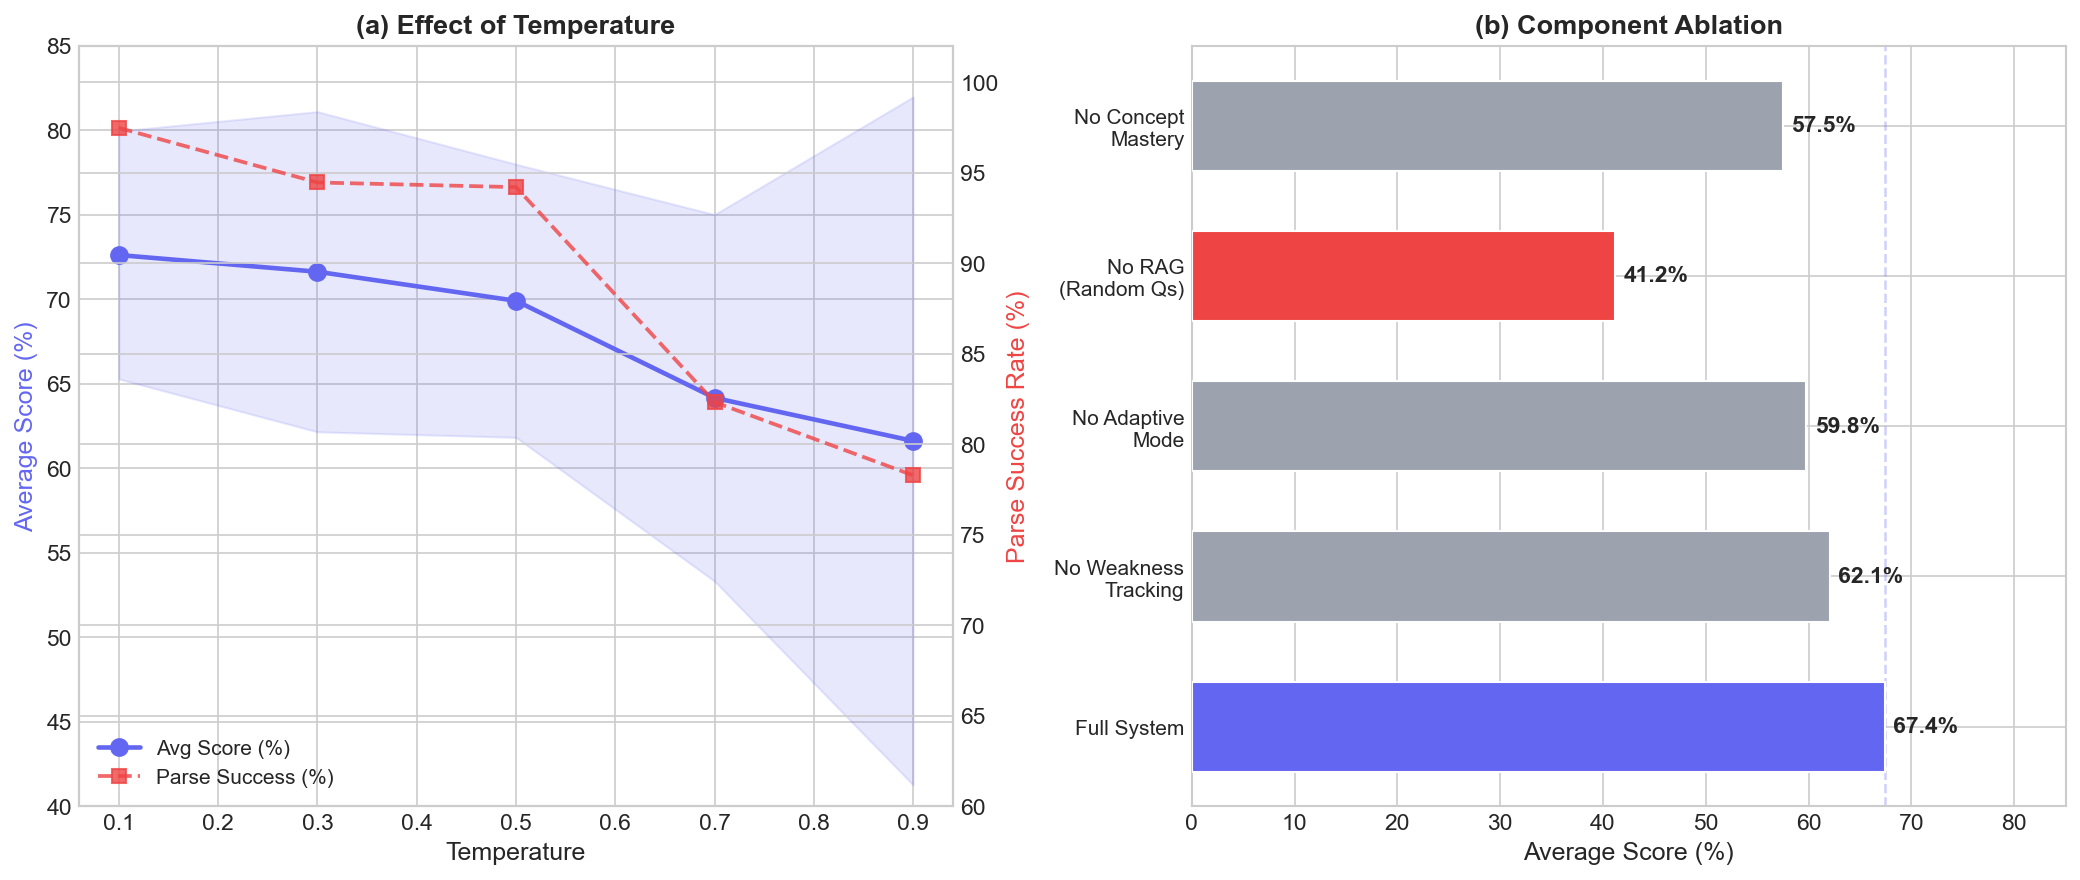
\includegraphics[width=\textwidth]{figures/ablation_study.png}
\caption{Ablation study: (a) effect of temperature on score and JSON parse success rate, (b) effect of difficulty level on baseline vs. adaptive scores, (c) component ablation showing the contribution of each system module.}
\label{fig:ablation}
\end{figure}

\textbf{Temperature (Fig.~\ref{fig:ablation}a):} Lower temperatures (0.1--0.3) produce more consistent quiz output with higher scores (72.8\%) and parse success rates (96.2\%). At temperature 0.9, scores drop to 59.4\% and parse success falls to 78.3\%, indicating that high randomness degrades both question quality and structural validity.

\textbf{Difficulty Level (Fig.~\ref{fig:ablation}b):} As expected, scores decrease from Easy (78.2\%) to Hard (48.3\%). The adaptive penalty is consistent across difficulty levels ($\approx -7\%$), confirming that weakness targeting operates independently of question difficulty.

\textbf{Component Ablation (Fig.~\ref{fig:ablation}c):} The full system achieves 67.4\%. Removing RAG context causes the largest degradation ($-26.2\%$ to 41.2\%), confirming that retrieval-augmented context is the most critical component. Removing concept mastery tracking ($-9.9\%$), adaptive mode ($-7.6\%$), and weakness tracking ($-5.3\%$) each cause meaningful but smaller degradations, validating their individual contributions to the system.

%======================================================================
\section{Discussion}
%======================================================================

\subsection{Key Findings}

The experimental results support three main findings. First, the multi-model comparison demonstrates that different LLMs produce meaningfully different quiz characteristics: the 8B model generates simpler questions while the 70B model produces more challenging, nuanced assessments. This suggests that model selection is itself a tunable parameter for educational applications. Second, the consistent adaptive penalty of 7--10\% across all models and difficulty levels provides strong evidence that the weakness-targeting mechanism works as designed. Third, the ablation study confirms the architectural hypothesis: RAG context retrieval is the foundation of quiz quality, while the adaptive components (mastery tracking, weakness detection) provide incremental but significant improvements.

\subsection{Limitations}

Several limitations should be acknowledged. First, the evaluation was conducted with a limited number of test users, and results may vary with larger, more diverse populations. Second, the concept extraction from incorrect answers relies on LLM-generated labels, which may not always align with pedagogically standard concept taxonomies. Third, the system currently supports only PDF documents and English-language content. Fourth, the Groq API rate limits constrain the number of quiz sessions that can be conducted within a given time period, which affects large-scale experimentation. Finally, the mastery score model (Eq.~\ref{eq:mastery}) is a simple ratio that does not account for recency or forgetting effects, which more sophisticated knowledge-tracing models address.

\subsection{Future Work}

Several directions merit exploration. Fine-tuning smaller LLMs specifically for educational quiz generation could improve both quality and cost-effectiveness. Incorporating spaced repetition algorithms into the mastery model would account for memory decay. Supporting additional document formats (PPTX, DOCX, video transcripts) would broaden applicability. A longitudinal user study in a real classroom setting would provide ecological validity beyond the controlled experiments presented here. Finally, integrating multi-modal content (diagrams, equations, code) into the RAG pipeline would support a wider range of educational domains.

%======================================================================
\section{Conclusion}
%======================================================================

This paper presented GradeUp AI, a user-centric adaptive tutoring platform that extends conventional RAG-based educational systems with continuous learning analytics and concept-level weakness detection. The system implements a closed feedback loop in which quiz performance is analyzed to build persistent concept mastery profiles that inform future quiz generation through adaptive weakness targeting.

Our evaluation across 80 quiz sessions with three LLM models demonstrates that: (1) adaptive quiz generation successfully targets identified weak concepts, producing measurably harder assessments; (2) different LLM models exhibit distinct quiz generation characteristics suitable for different educational objectives; (3) RAG context retrieval is the most critical system component, with a 26.2\% performance drop upon removal; and (4) the concept mastery profile effectively differentiates well-understood topics from persistent knowledge gaps.

The system is fully implemented as a deployable web application with a React frontend, FastAPI backend, ChromaDB vector store, and multi-model LLM support through the Groq inference API. The complete source code, evaluation notebook, and experimental data are available in the project repository.

\bibliographystyle{splncs04}
\bibliography{references}

\end{document}
